%!TEX TS-program = xelatex
%!TEX encoding = UTF-8 Unicode
\documentclass[11pt, a4paper]{article}
\usepackage{my-additions-x}

% my macros
\def\code{\texttt}
\def\tred{\texttt{TrEd}}
\def\ntred{\texttt{N-TrEd}}
\def\seman{\texttt{SemAnn}}
\def\semlex{\texttt{SemLex}}
\def\astst{$\ast$.st}
\def\sdata{s-data}
\def\stn{st-node}
\def\sn{s-node}
\def\tn{t-node}
\def\stf{st-file}
\def\sf{s-file}
\def\tf{t-file}
\def\mwe{MWE}
\def\Mwe{multi-word expression}
\newcommand\Sref[1]{Section~\ref{#1}}

\title{Thesis Notes}
\author{\textsc{Pavel Straňák}}

\begin{document}
\maketitle

%%%%%%%%%%
\section*{Motto}
\begin{tabular}{@{} lp{11cm} @{}} % @{} removes default spaces
Frasier: & ``How was your hunting trip?''\\
Martin: & ``Came home empty handed.''\\
Frasier: & ``Oh dear; I guess that means for the next several weeks we'll hear your grouse about the grouse and carp about the carp.''\\
Niles: & ``You've been working on that, haven't you?''\\
Frasier: & ``Well, there was traffic.''\\
 & \raggedleft\emph{Frasier, Season 9, Part 3}\\
\end{tabular}

\section*{Idioms}
Even ``non-compositional'' idioms are actually (originaly) metaphorical or methonymical.  Even though sometimes it is hard to see that. At other times a speaker may forget that rather straightforward metaphoric aspect:

\begin{quote}
Barack Obama accused his Republican rivals of stirring a controversy over a comment he made about putting “lipstick on a pig.” \emph{(NY~Times, 11.~September 2008)}
\end{quote}


%%%%%%%%%%%%%%%%%%%%%%%%%%%%%%%%%%%%%%%
\section{PDT 2.0}\label{PDT}
In the Prague dependency treebank version 2.0 (PDT, ) there are several functors that refer to multiword expressions (MWEs) in one way or another. There are also two technical lemmas \texttt{\#Idph} and \texttt{\#Forn} that identify roots of subtrees representing MWE's. Tectogrammatical annotation is described in detail in~\citet{mikulova:2006}.

There are currently two graphical search engines for PDT: Netgraph \citep{mirovsky:2009} and TrEd \citep{pajas:tred}. Both have their respective benefits, but since TrEd is considerably faster due to its use of an SQL database backend \citep{pmltq}, we have used TrEd for all the examples in this work. We also give the search queries using the PML Tree Query language designed by \citet{pmltq} where appropriate.

%%%%%%%%%%
\subsection{Foreign Phrase: \code{t-node [t\_lemma = \#Forn]}}\label{PDT:Forn}
Foreign Phrase seems to be overused and its overuse seems a bit arbitrary. \\
- jmena firem jsou nekdy forn, nekdy ne. (dohledat)\\

%%
\subsubsection{Foreign phrases with just one t-node}
There are 34 occurrences of this construction in the PDT~2.0. Counting them is as easy as writing a query in Figure~\ref{fig:tq-forn1} and extending it with this filter: \code{>>count(\$n)}.

\begin{wrapfigure}{r}{0.32 \textwidth}
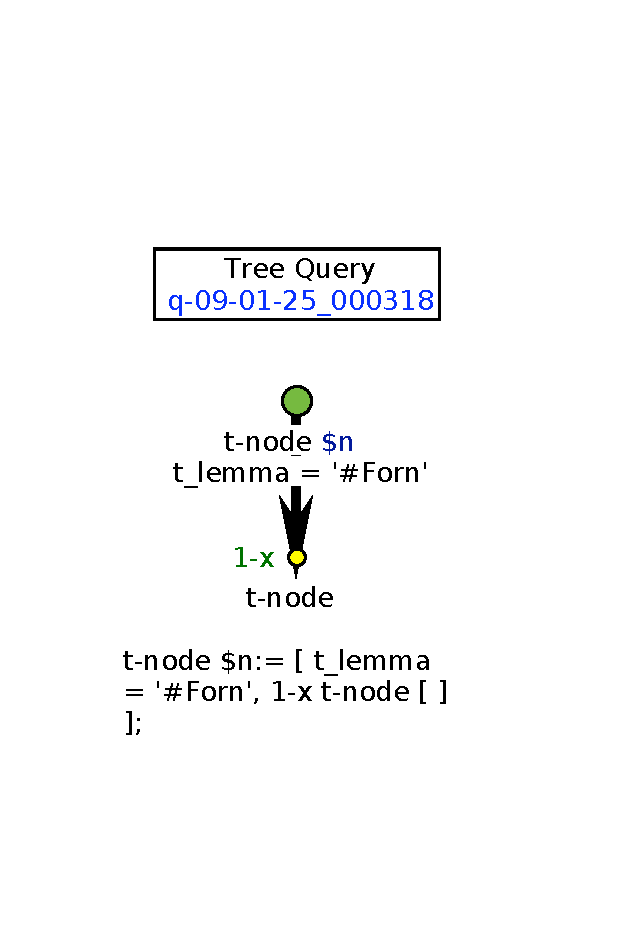
\includegraphics[width=0.3 \textwidth]{images/vyhledavky/query-forn-1-x.pdf}
\caption{PML-TQ search query for single-node foreing phrases}
\label{fig:tq-forn1}
\end{wrapfigure}

In case of the bibliographic reference in Figure~\ref{fig:forn-biblio} there is coordination of three foreign phrases corresponding to the parts of a bibliographic reference annotated, but the reason for this is not very clear. After all, the point of annotating foreign phrases as simple lists with a \code{\#Forn} node as a head was to make no assumptions about these pieces of a text \pageref{pdt-t-man:300}.  \\
- je to kvuli te interpunkci???

\begin{figure}[h]
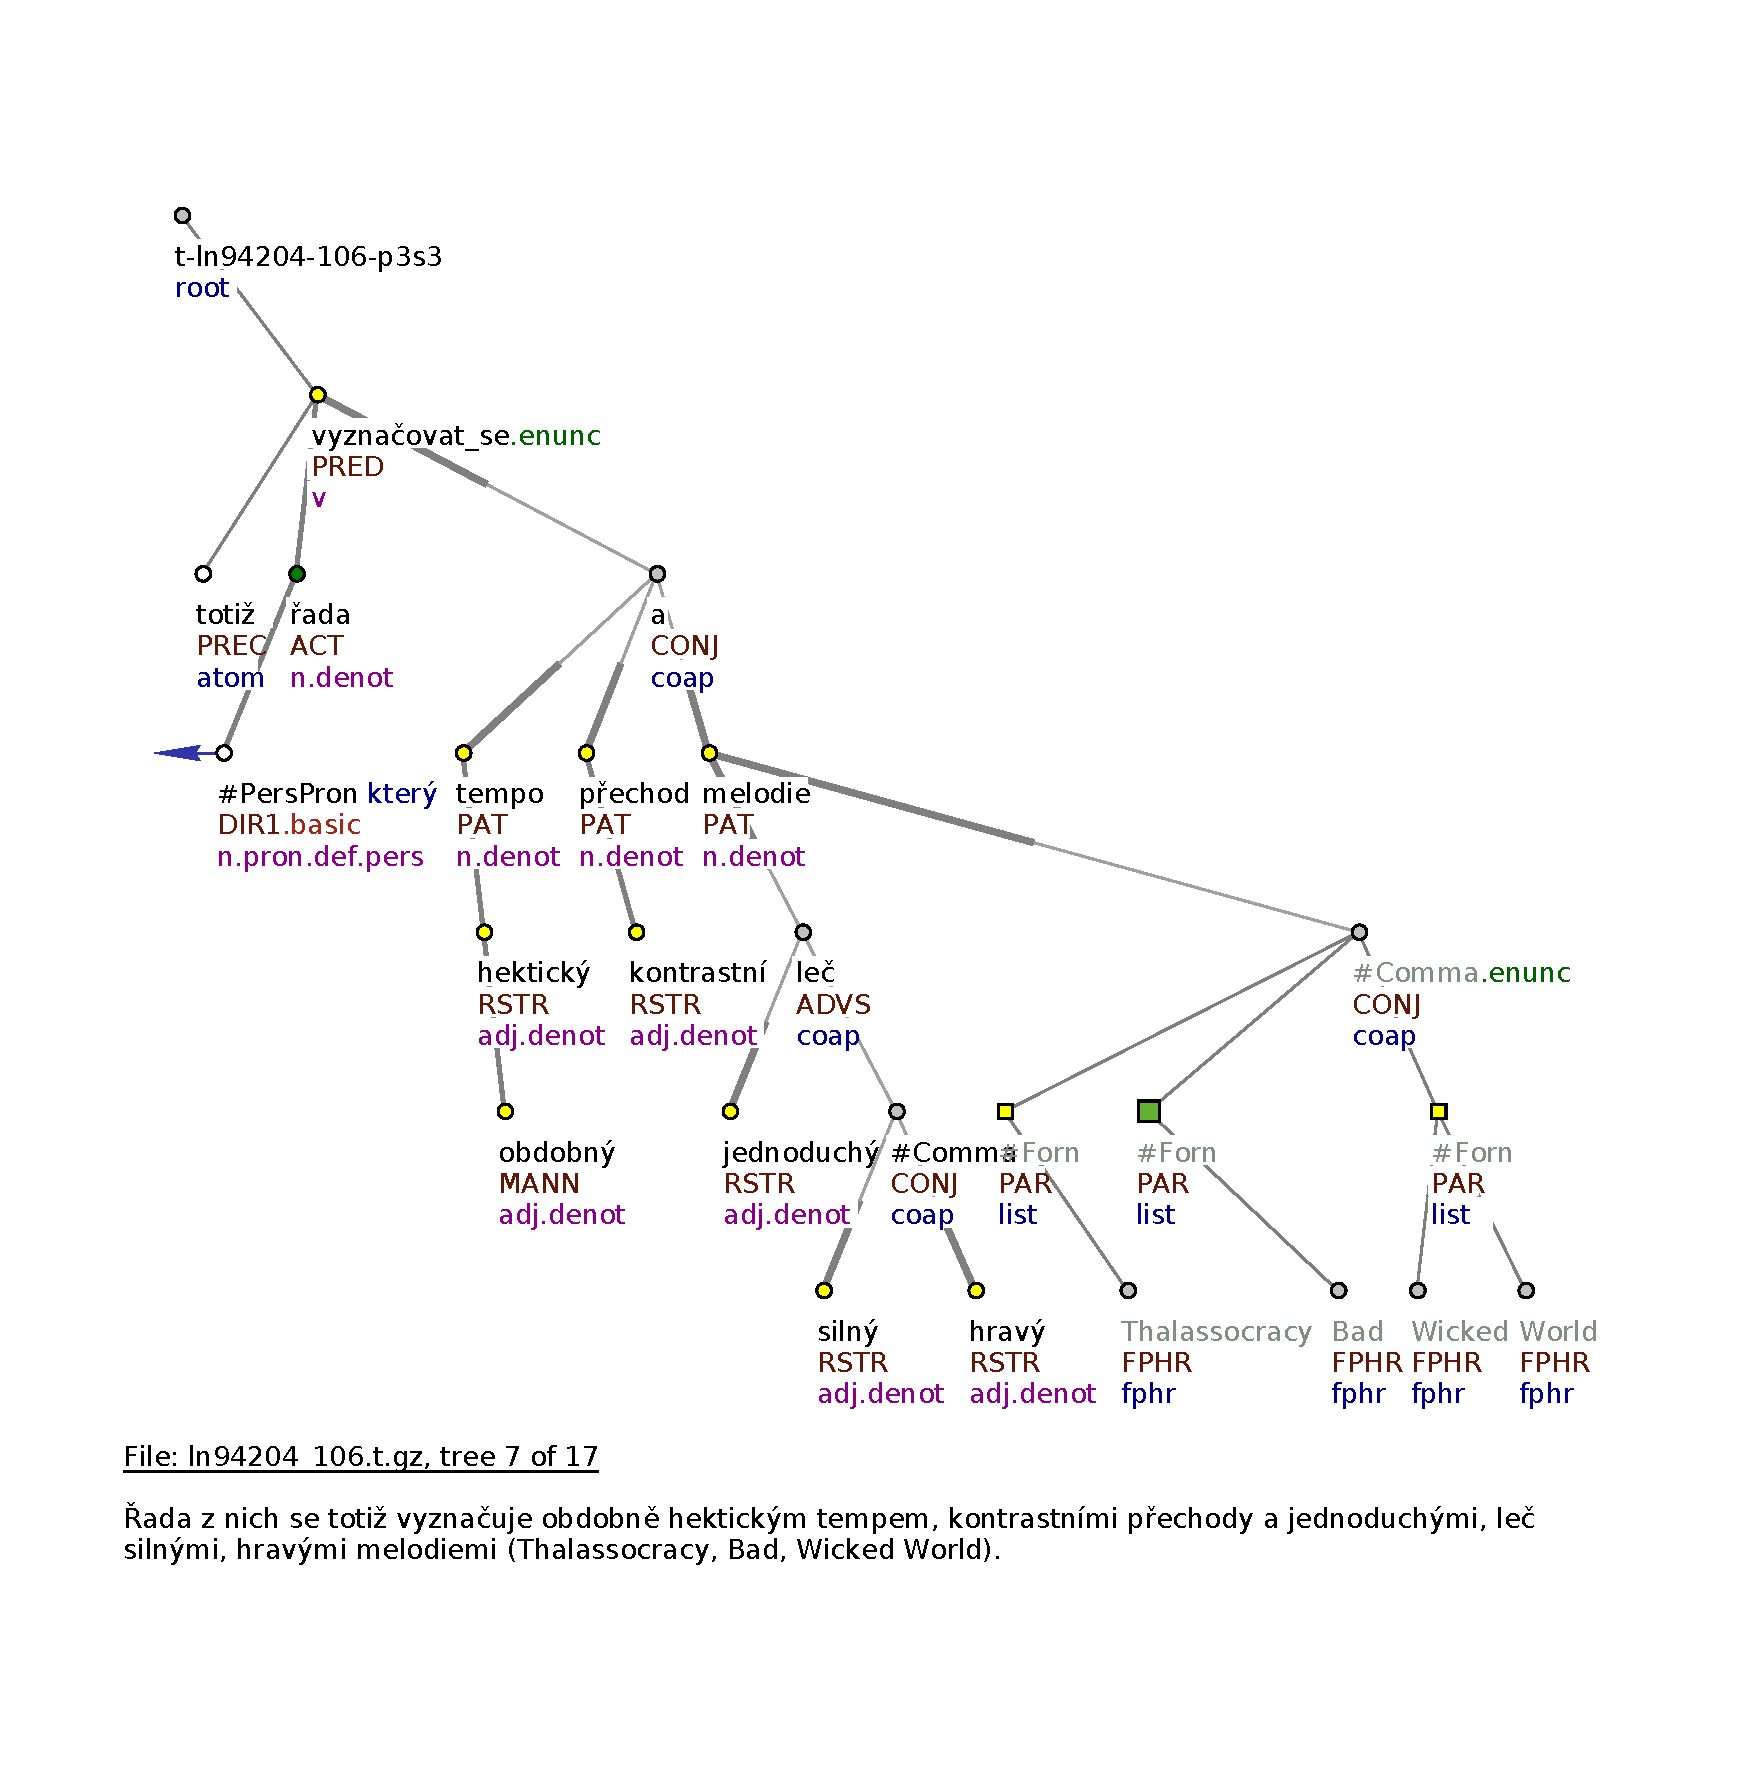
\includegraphics[width=\textwidth]{images/vyhledavky/forn-coord1x-biblio.pdf}
\caption{A bibliographic reference analysed as a coordination of three foreign phrases}
\label{fig:forn-biblio}
\end{figure}

Names of companies seem to be distinguished more by the country of origin then by any linguistic reasons, as demonstrated in Figure~\ref{fig:forn-firmy}. As far as linguistic criteria are concerned, Chemapol and Inekon are as foreign as Agip or Total. However the first two are, or at least were,%
\footnote{At the time of writing this thesis Chemapol is owned by another international company, which only emphasises vagueness of this distinction} %
%
Czech companies, while those in the latter group have a foreign origin.

\begin{figure}
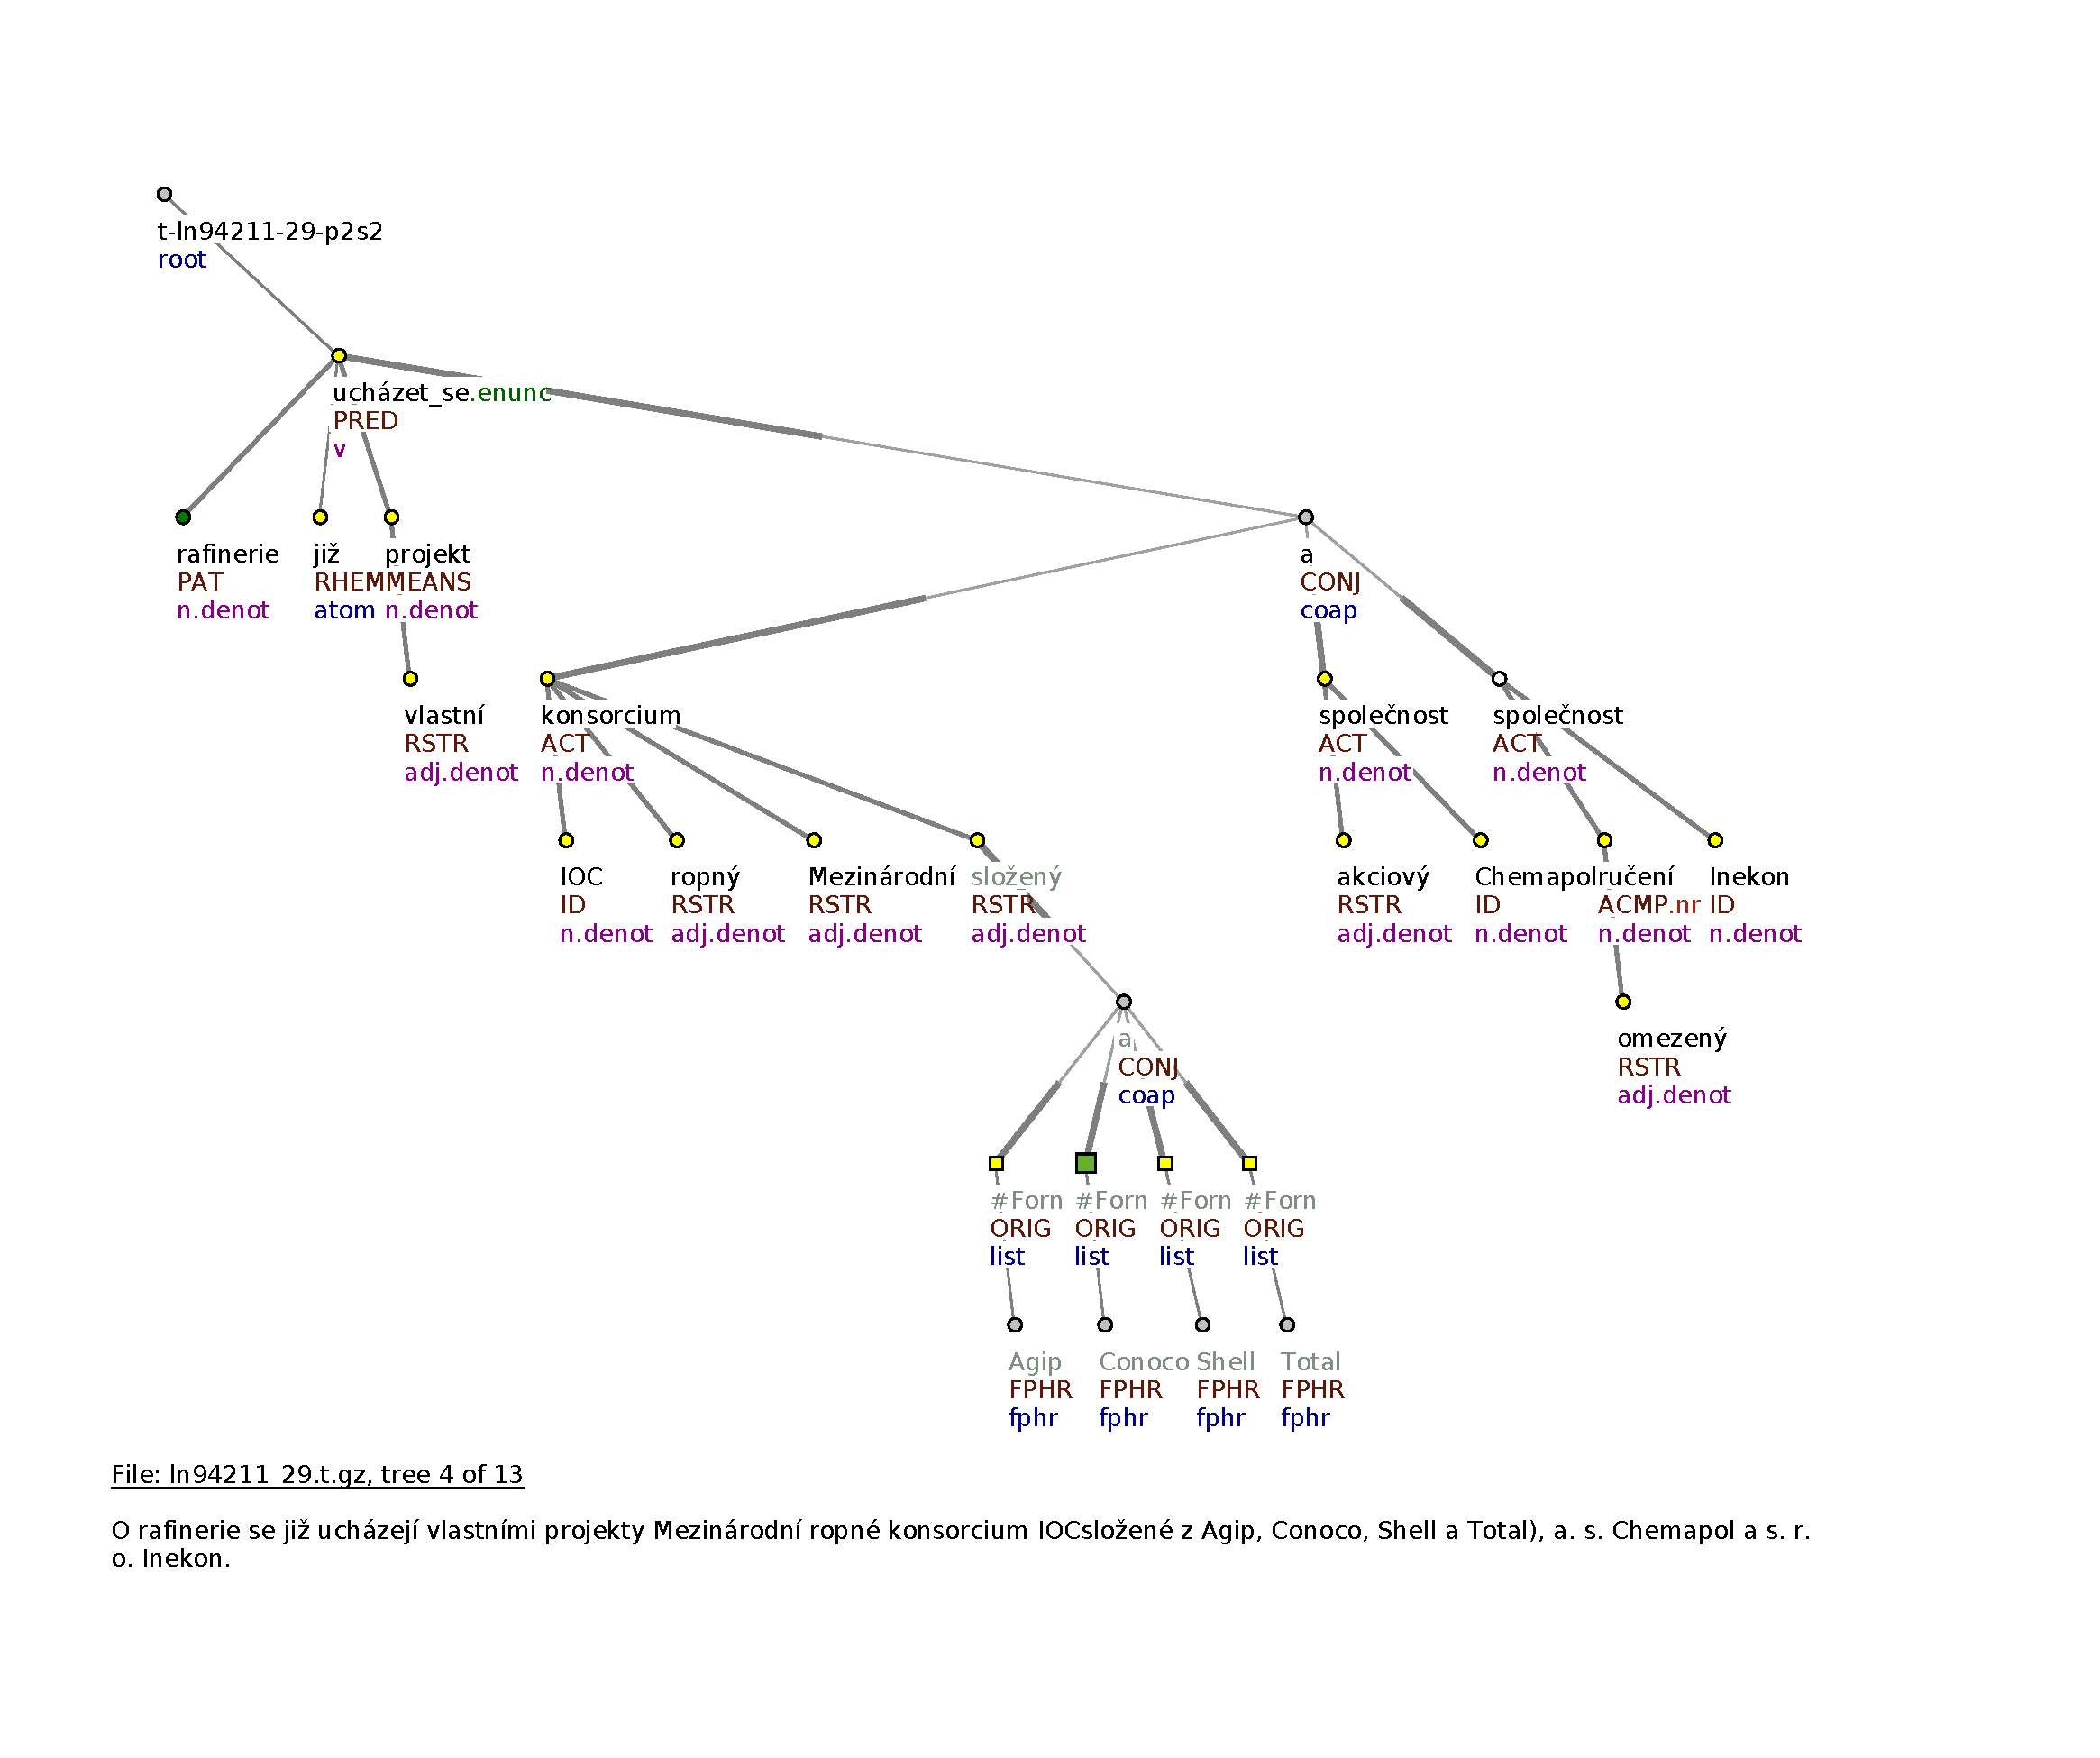
\includegraphics[width=\textwidth]{images/vyhledavky/nazvy-firem.pdf}
\caption{Annotation of Czech and foreign company names}
\label{fig:forn-firmy}
\end{figure}

%%%%%%%%%%
\subsection{CPHR}
There are 76 occurrences of {\tt CPHR} nodes, whose head verb is not its parent, but only effective parent, in 40 sentences. See Figure~\ref{fig:tq-echild} for the query and Figures~\ref{fig:cphr-echild} and~\ref{fig:cphr-echild2} for examples.
\begin{wrapfigure}{r}{0.32 \textwidth}
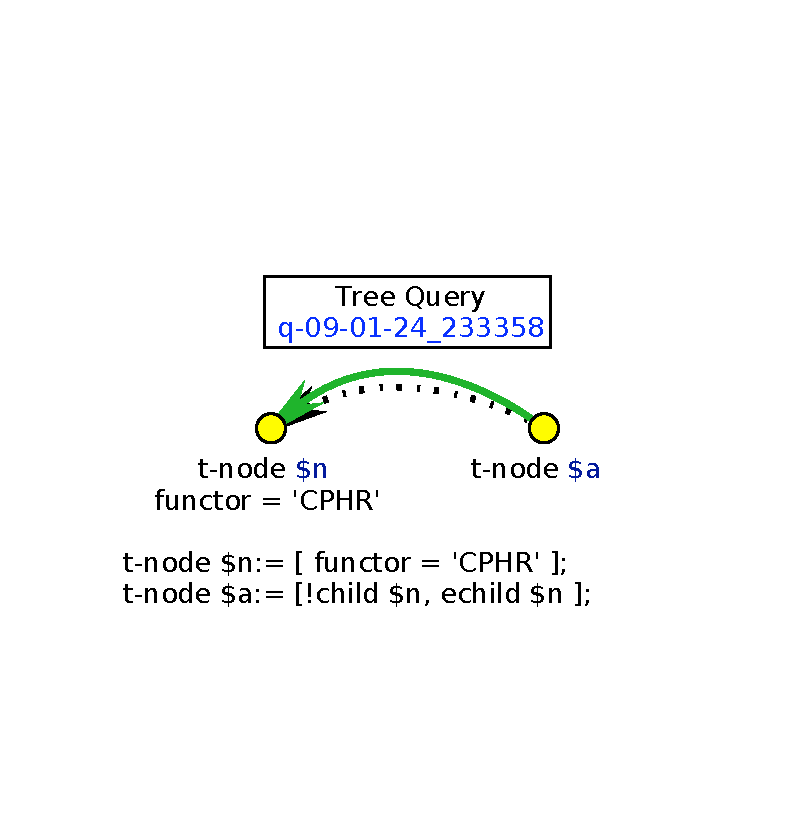
\includegraphics[width=0.3 \textwidth]{images/vyhledavky/query-echild.pdf}
\caption{PML-TQ search query for CPHR nodes, whose effective parrent is not its parent}
\label{fig:tq-echild}
\end{wrapfigure}

\begin{figure}[h]
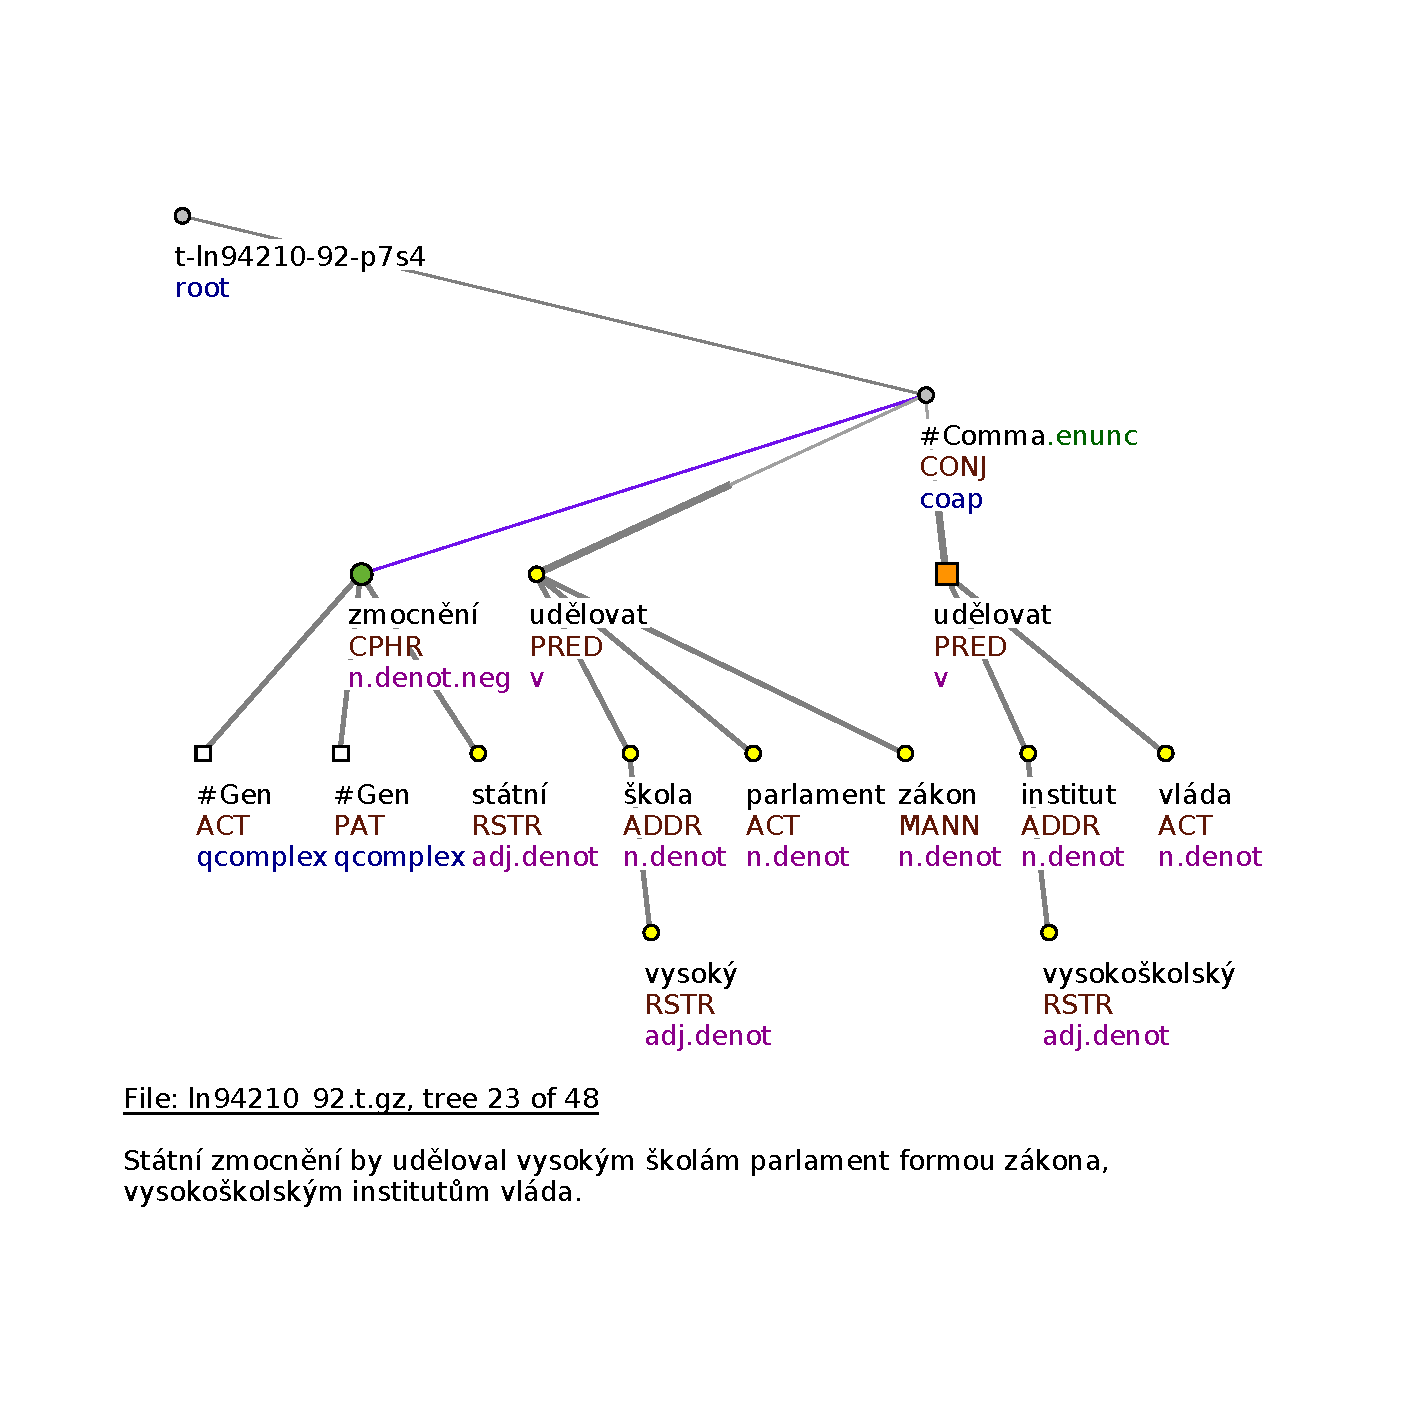
\includegraphics[width=0.8\textwidth]{images/vyhledavky/cphr-echild.pdf}
\caption{Coordination of verbonominal idioms, where the verbal parts are further ???rozvite }
\label{fig:cphr-echild}
\end{figure}

Figure~\ref{fig:cphr-echild2} shows on the other hand a coordination of two V-N idioms with the same verbal part.
\begin{figure}[h]
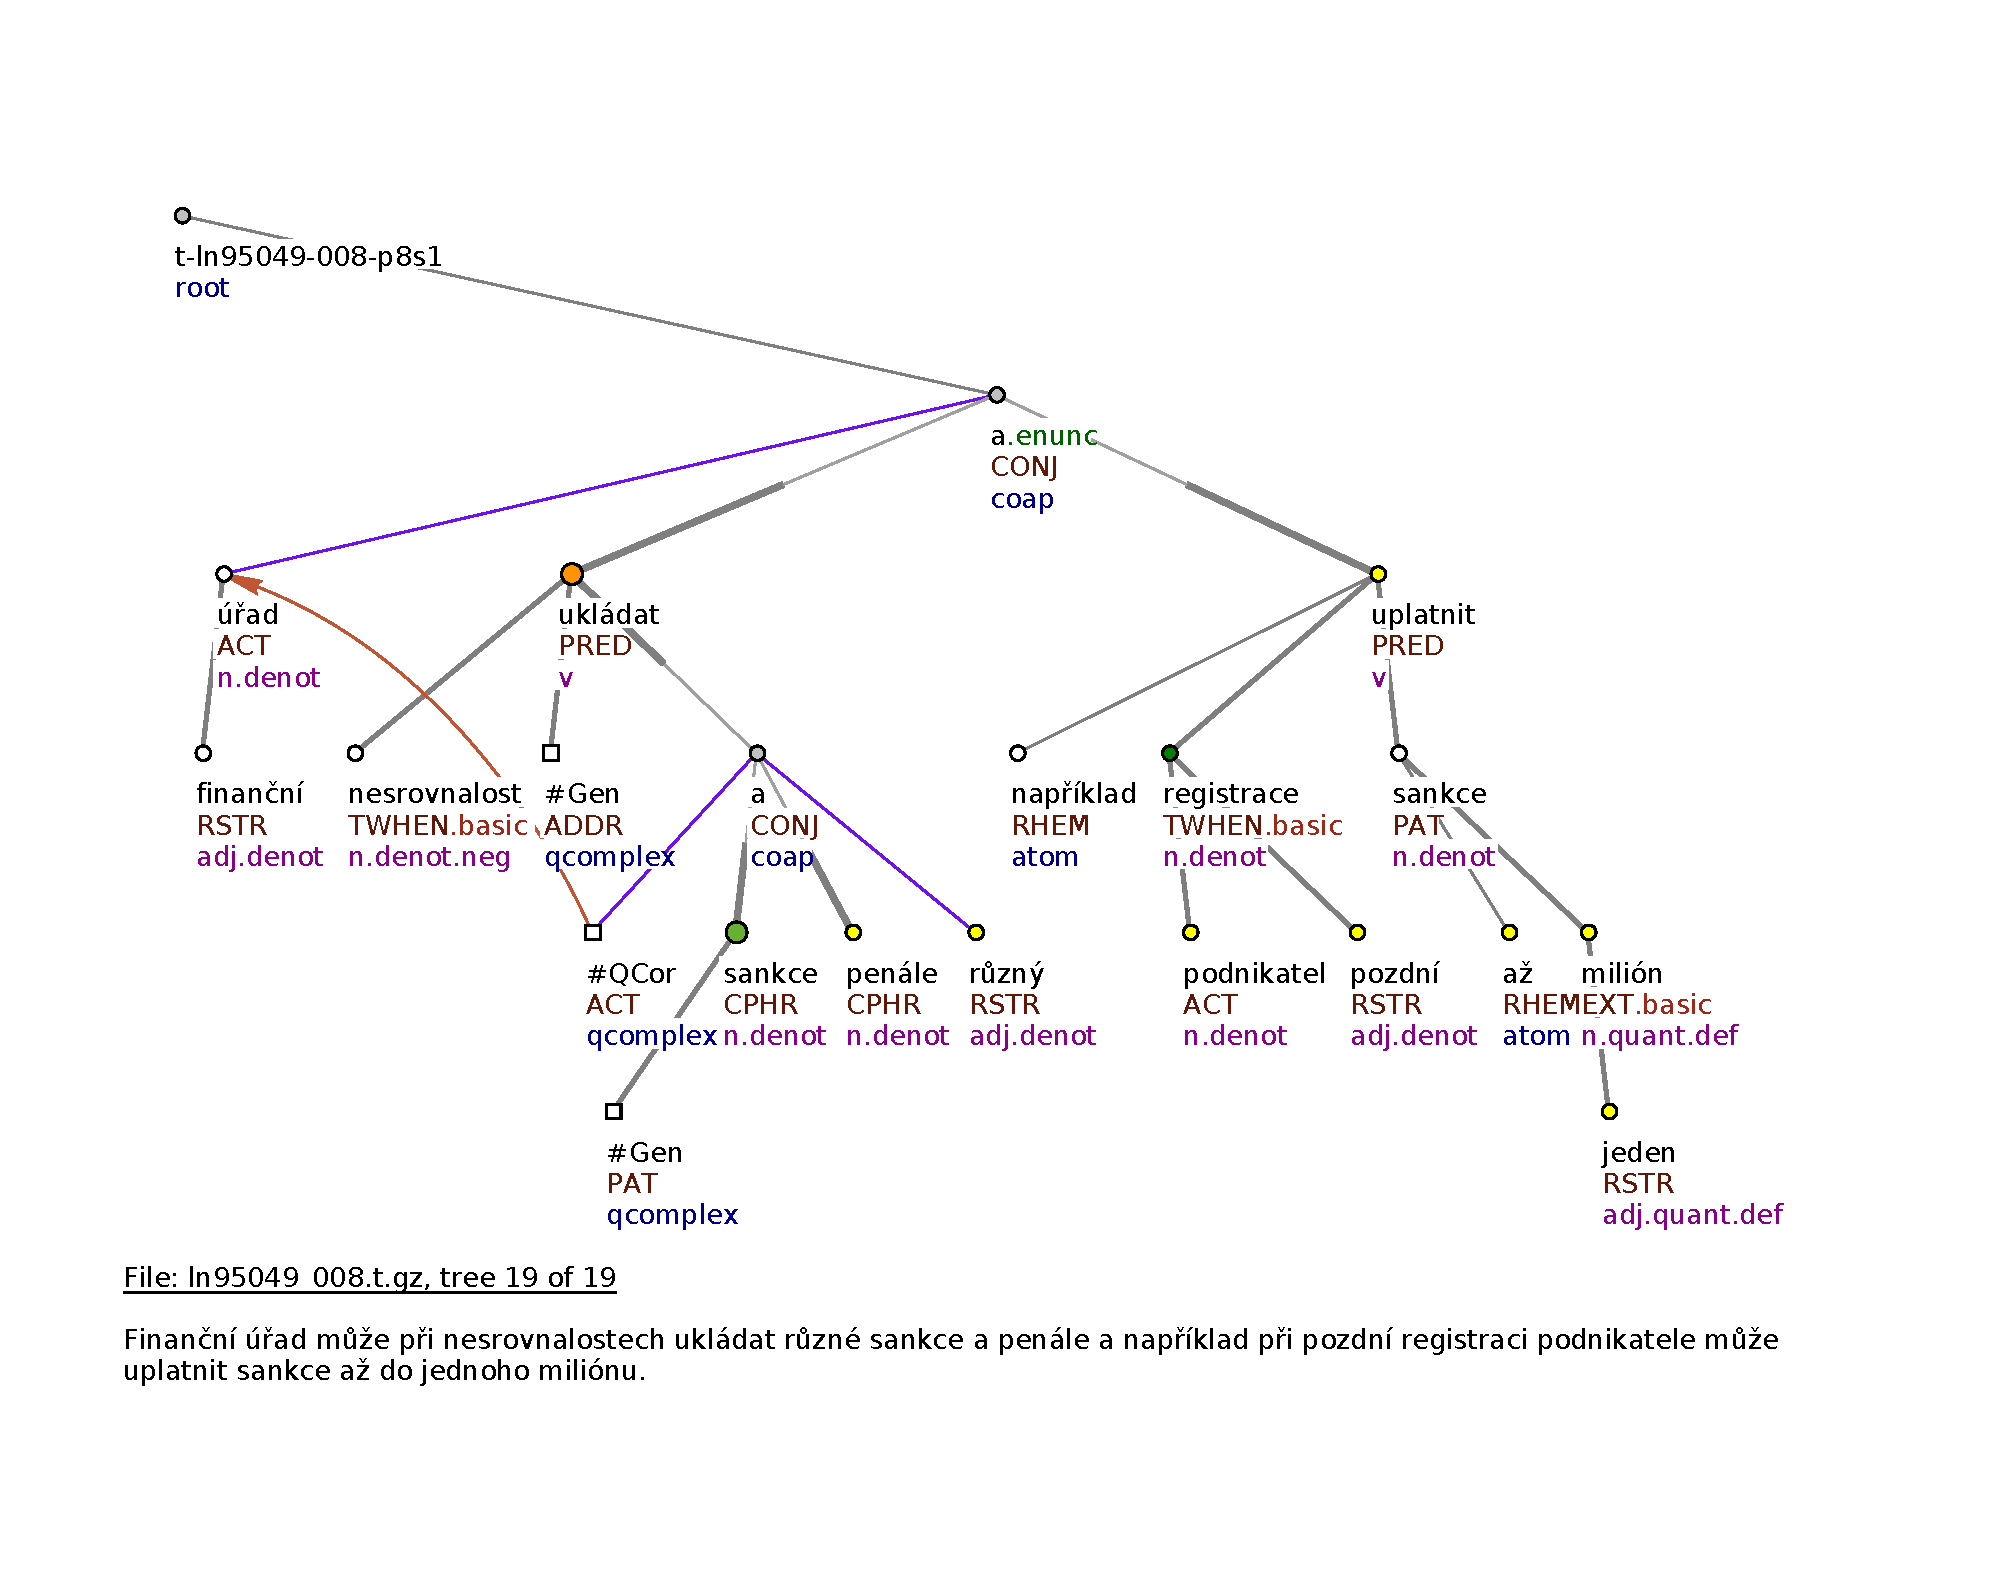
\includegraphics[width=\textwidth]{images/vyhledavky/cphr-ukladat-sankce-a-penale.pdf}
\caption{Coordination of two idioms starting with the same verb}
\label{fig:cphr-echild2}
\end{figure}

\newpage
\section{Notes}

{\em``Prokopnout pětku''} -- prokopnout [trestný kop after scoring] pětka -- ellipsis crossing into pragmatics(?), because it is {\em not} an ellipsis of some exact linguistic construction, but rather an ellipsis of a situation which everyone in the discourse understand.  

``Návrh / novela Zákona na ochranu osobních údajů''  $$((\mathrm{návrh} \lor \mathrm{novela}) | \mathrm{zákon} \lor \mathrm{předpis})$$
-- lexikální funkce?? \citep{wanner} ?

\subsection{Missing t-nodes in \code{coord}s}
``\textit{První} a druhá světová válka'' apod. -- the word ``První'' is an ellipsis of ``První světová válka''. The ellided t-nodes that should had been newly established were not, however, which left us two options, either annotate a single-word (and single-node) expression as an instance of a multi-word lexeme, or annotate the words ``světová válka'' that occure in the text as being a part of both expressions. We decided for the first, because the agreement on ellipses is fairly high in this type of coordinations.

% !TEX root = ../disertace.tex
%!TEX encoding = UTF-8 Unicode

\chapter{\sdata}
\section{The design and the PML schema}
\sdata\ means s-layer PML files and the PML schema of these files. The idea behind \sdata\ design is to have a simple way to store additional ``sense'' annotations over any layer of PDT. The annotations are stored as a set of ``sense'' nodes. Each s-node contains a link to a sense repository (annotation lexicon) and a set of references to nodes (m-, a- or t-) that correspond to an instance of the sense. An \sf\ is thus basically a very simple flat list of \sn{}s. It does not contain any trees. A single \sf\ can only reference a single PDT file: either tectogrammatical, or analytical, or even morphological layer can be used, but references to different layers cannot be mixed in one s-file.

The design of \sdata\ is quite universal. S-files can be used to provide additional annotations over any PML files that contain nodes with IDs. The sense repository (annotation lexicon) can be any dictionary that provides IDs for the entries. The tools used in our annotations mostly expect PDT PML or the particular \sf{}s that we have used, but that is mostly for convenience. Should the need appear to adapt the workflow a different corpus represented by PML files and a different annotation lexicon, the changes required would be rather minor.

\section{Visualisation}
There are two basic ways to view st-nodes: in \seman\ or in \tred. Both of these need to use the ``t-a-m-w-'' PDT files to display the sentence and/or the tree for each sentence and then they read the \stf\ to add the information about \stn{}s. The \stn{}s are displayed as colour boxes or bubbles over the words in a sentence or nodes in a tree in \seman\ or \tred\ respectively.

\subsection{Visualisation using \seman}
The visualisation of annotated files in \seman\ has the advantage of showing whole text with all the \mwe{}s clearly marked in a single glance. Integration of the SemLex browser is also beneficial, because it allows fast and convenient lookup of annotated \mwe{}s in \seman. Details of \seman\ interface are described in \Sref{sec:seman}. 

There are, however, also some drawbacks of this ``full plain text of an article'' approach: 

\section{\tred\ extension}
\tred\ has a powerful mechanism that allows it to be extended for new tasks. We developed an extension \texttt{pdt-t-st} that allows to see MWEs as graphically marked groups of tectogrammatical nodes. 

 Main features of the extension:
 \begin{itemize}
\item
Merges the \stf{}s into \tf{}s and allows to display these enriched tectogrammatical trees.
\item
Types of annotated MWEs (i.e. types of NEs and \semlex\ entries) are distinguished with the same colours that were used in \seman\ during annotations. This allows not only for easily seeing NE types, but also easily spotting annotators' disagreement on them. 
\item
Allows to merge annotations of several annotators into one \tf. 
\item
Each annotator's MWEs have a unique raster. It is thus easy to spot annotators' partial or full disagreement not on types of MWEs, but also on their spans.
\end{itemize}

 There are two ways to merge the \sdata\ and \tdata: 
 \begin{enumerate}
\item
Merge on opening the \stf\ in \tred, and
\item
Static merge that produces the merged \verb=*.t.mwe.gz= file. 
\end{enumerate}
The dynamic merging is done using a newly developed feature of \tred\footnote{Developed by Petr Pajas} that allows to apply arbitrary perl transformations on the input data. Thus we open the \stf, use the mechanism of extensions to activate our extension by identifying the \stf\ as data the extension can process and call our transformation. The transformation requires a \tf\ annotated by this \sf\ to be present in the same directory. The \tf\ and \sf\ are parsed, and for each \stn\ we find a tectogrammatical tree that includes \tn{}s annotated (i.e. referenced) in this \stn. When we have a root of the correct t-tree, the \stn{}s are basically added into an attribute \texttt{mwes} of this t-root. The attribute is rather complex, because it contains lists of \stn{}s for all annotators that annotated any \stn{}s in this tree. Some small transformations of \stn{}s are needed, as well as creation of some new XML nodes, to represent the information from \sf{}s in the \tf{}s properly. For all the details inspect the code of \verb=$pdt_t_st/libs/SDataMerge.pm=.
%!TEX root = ../disertace.tex
%!TEX encoding = UTF-8 Unicode

\chapter{\seman}
\label{sec:seman}
The annotation tool \seman\ is written in Perl 5\footnote{\url{www.perl.org}; \url{dev.perl.org/perl5}} with Perl/Tk\footnote{\url{http://search.cpan.org/~srezic/Tk-804.029/}} GUI toolkit. The annotation tool depends on working installation of \tred, specifically its unix installation, because it uses \texttt{nTrEd} for efficient execution of \tred\ scripts in the background. \texttt{nTrEd} however, unlike \tred\ itself or \texttt{bTrEd}, does not work on Windows.% because it uses unix sockets.

% sem-ann screenshot 
\begin{figure}[htbp]
   \centering
   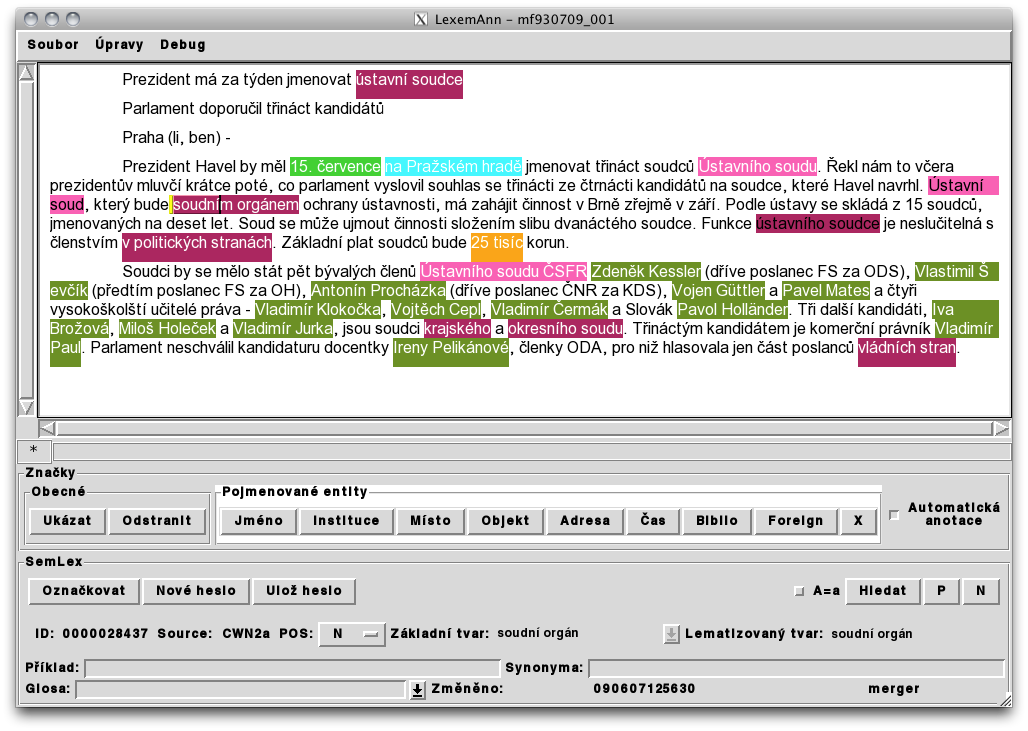
\includegraphics[width=.9\textwidth]{images/sem-ann2.png} 
   \caption{An annotated document in \seman. the yellow ``selection tag'' is barely visible on the word \pr{soudním}, because over a  different colour tag, selection has just a bezel. The \semlex\ entry that is displayed in the Semlex-part of the UI -- \pr{soudní orgán} -- is the one used to annotate the selected word. The black font colour in two tags distinguishes automatically pre-annotated MWEs.}
   \label{fig:seman-gui}
\end{figure}

\seman\ itself is composed of several main parts:
\begin{itemize}
  \item The main application file \code{sem-ann.pl} mostly implements the application frontend. It implements the GUI, loads an \sf, a \semlex,  and a log file for this \sf, if it had already been annotated. Then it takes care of all the interaction with the user and writes \sf, \semlex, and a log file.
  \item \ntred\ backend that is used to 
	\begin{itemize}
	  \item generate surface sentences from tectogrammatical trees in \tf{}s that are then displayed in the \seman\ GUI,
	  \item perform all the on-the fly pre-annotations (\Sref{sec:annot:pre})
	\end{itemize}
A \tred engine without a GUI with a few modifications aimed towards batch processing is called \btred. \ntred is essentially a modification of \btred that allows it to run as a daemon and process scripts over a network. We opted for \ntred, even though we ran it locally, because it can run as a daemon, thus eliminating a significant startup penalty of \btred. What we call ``\ntred\ backend'' is thus the running \ntred\ instance itself (that is started by the \seman\ during start-up, if there has not been a running instance detected), and the scripts used to generate the sentences that are displayed in \seman\ and to pre-annotate MWEs using their tectogrammatical tree structures.\footnote{these scripts were written entirely by E. Bejček~(\citeyear{bejcek:2010}).}
  \item The module \code{SemLex.pm} is used to read, save, query, and edit \semlex.
    \item The module \code{SemLex\textunderscore{}heslo.pm} implements the \semlex\ entry: its structure, attributes and accessors.
  \item There is also a suite of miscellaneous scripts mostly for validation of annotated data, comparing and merging multiple annotations, merging annotators' \semlex{}es, computing reliability of annotations, and other small tasks related to annotation and managing the annotated data and \semlex{}es.
\end{itemize}

%%%%%%%%%%%%%%%%%%
\section{User interface}
\label{sec:seman:gui}
The user interface (shown in \Fref{fig:seman-gui}) is divided three main parts: The text widget displaying the annotated text, a row of buttons to create annotations by NE tags, show info on annotations, or remove tags, and an editor of \semlex. 



%%%%%%
\subsection{Text widget}
\label{sec:text-widget}
The text, displayed for the annotator, is generated from the tectogrammatical trees (using also information from lower layers). That is, why for each document to be annotated, all the PDT files must be present ( t-, a-, m-, and w-layer). 

It is possible to generate the surface (plain text) sentence from a t-tree using the `built-in' function \verb=PML_T::GetSentenceString($root)=. Such a sentence is complete, correct, has correct spacing around punctuation, but it contains no relation to the t-layer anymore. And we want to keep this connection in order to be able to annotate the t-nodes, not just words \see{sec:annot}. Thus Eduard Bejček wrote the script \url{get_sent_t-layer.btred}, that creates a representation connecting words in a sentence with tectogrammatical IDs of the t-nodes from which these words are generated. This representation is actually input into the text widget and everything but the words is hidden from the annotators' view. \emph{The tecto-IDs are then what gets really annotated, \emph{using} the words.} The full representation can, however, be displayed using Debug menu commands. It is shown in \Fref{fig:seman:hidden} in comparison to the ``plain text'' as normally displayed (with no actual annotations to keep the view simple).

%% comparison of plain text and the same with hidden text -- screenshots%%
\begin{figure}[htbp]
   \centering
   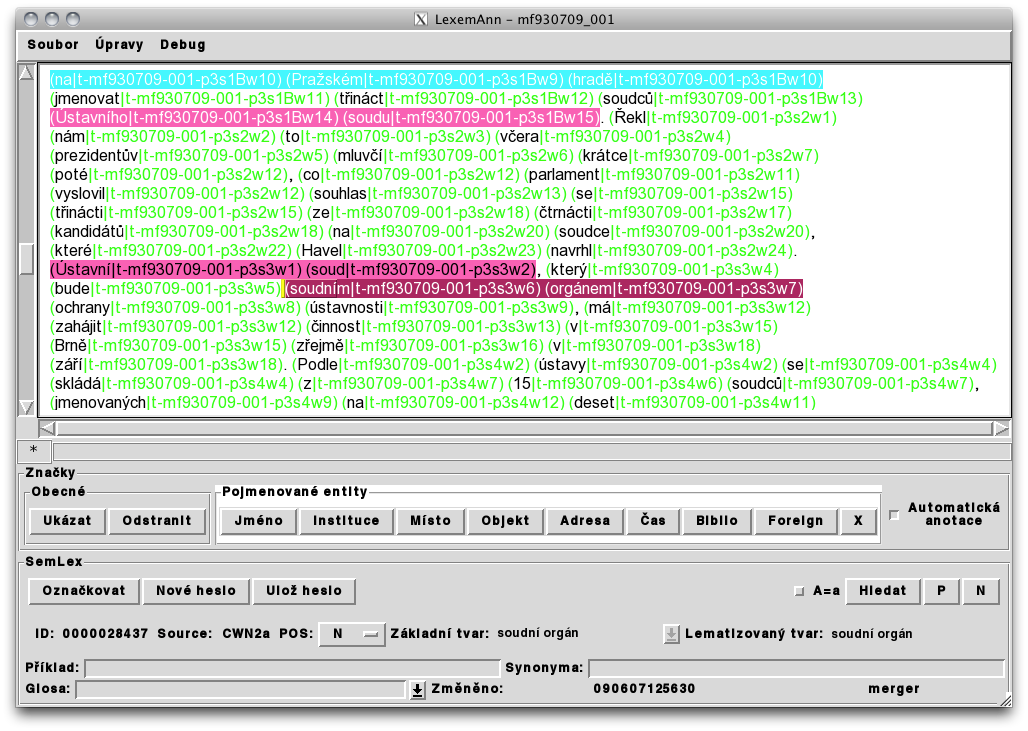
\includegraphics[width=.95\textwidth]{images/hidden-text2}
   \caption{Comparison of the plain text, as normally displayed, and the underlying representation that is used to relate the actions of annotators who mark words, to the references to tectogrammatical nodes that are actually saved in the annotation files.}
   \label{fig:seman:hidden}
\end{figure}



%%%%%%
\subsection{Annotation buttons}
The row of buttons below the text widget and the status bar is rather straightforward: 

The first group (from the left) contains two buttons that are connected to general commands used for all annotations (NEs and other \semlex\ entries alike). The first button shows a tag (i.e. the corresponding \semlex\ entry), on the word in focus (the word that is selected, or in which the cursor is placed). The second button removes the tag on the word in focus.

The second group of buttons simply creates NE tags over the selection. 

The last check button toggles the on-the-fly pre-annotation of other instances of the same MWE that annotator annotates, in the rest of the text (pre-annotation type~\ref{pre-on-annot}, see p.~\pageref{pre-on-annot}).



%%%%%%
\subsection{SemLex editor}
The \semlex\ editor and browser (see the lower part of \Fref{fig:seman-gui}) simply displays SemLex entries, allows to edit them, or to search SemLex by basic or lemmatised forms (see~\Fref{fig:semlex-search}), and browse the search results (using their basic forms). There is also a function to annotate the selected words (t-nodes) with the current SemLex entry. It is mapped simply to the return/enter key, once the focus moves from the SemLex part of the GUI to the text widget.

The attributes of an entry that are displayed include the basic and lemmatised form of an entry, its ID and source, example of usage, synonyms, if present, and a gloss. There is also a time stamp and a signature of the last modification. The attributes of a SemLex entry are explained in detail in \Sref{sec:semlex:entry}.

The search string is by default matched as a substring, and there is a check box to toggle case sensitivity. However when needed (and in case an annotator has the knowledge), full Perl regular expressions can be used. 
\begin{figure}[htbp]
   \centering
   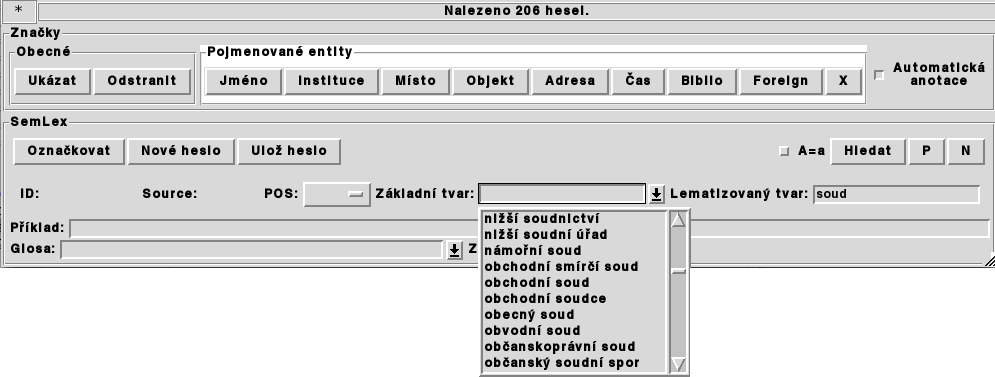
\includegraphics[width=\textwidth]{images/semlex-search}
   \caption{A result of a search in SemLex by a substring of the lemmatised form: 206 entries were found (see the status line at the top). Browsing the basic forms of the results.}
   \label{fig:semlex-search}
\end{figure}

%%%%%%
\subsection{General UI remarks}
Inspired by command mode of modal text editors and by some annotation regimes of \tred, we made all the annotation commands single-letter. That was made possible by making the text read-only. Since the letters are not used for input, they can be mapped to commands. All the command (and so the buttons) are named (in Czech) in such manner, that their first letter can be mapped to perform the command. Only the command for removing annotation is mapped to the capital letter (`O' for `odstranit') for safety reasons.


%%%%%%%%%%%%%%%%%%%
\section{Annotation logs}
\label{sec:logs}
An important, and as far as we know unique, feature of \seman\ is the design of annotation logs. As soon as an \sf is loaded in \seman, a \verb=*.st.log= file is created and every action taken henceforth, that modifies the \sf, is logged, together with a timestamp. 

Logs are saved in YAML format and timestamps are human readable on purpose. Thus it is easy to visually inspect the logs in case of problems with sf{}s, e.g. data corruption. It was helpful on several occasions. However the main point of logs is different.

Logs are a source of valuable information that can provide an insight into what is actually going on during annotation. Analysis of logs together with s-files can help estimate the real cost of annotations, which we have done during annotations to some extent, by estimating speed of annotations \see{sec:time-analysis}. 
But the analysis can go further and, to formulate the problem in economic terms, try to examine in general what factors influence the price of a (correct) tag. What is the relation of speed, length of work intervals, time of day, order of processing of the file, and other factors? We give only a very brief glimpse of one of the factors -- speed of annotations in \Sref{sec:time-analysis}, but in our opinion thorough statistical analysis of log files is an important source of information also for future annotation projects. \xx{Presunout odstavec do casove analyzy ve Future Work?}

The log files are however useful also directly to annotators during their daily work, because they provide information necessary for persistent undo and redo. Even when the file has been partially annotated long time ago, an annotator can review the last steps taken and continue with more information.

\bibliographystyle{plainnat}
\bibliography{Bibliografie}
\end{document}